\documentclass{memoir}
\usepackage[utf8]{inputenc}
\usepackage{amsmath,amsfonts,amssymb}
%\usepackage{caption}
\usepackage{subcaption}
\usepackage{tikz}
\usepackage{graphicx}
\usetikzlibrary{calc}
\thispagestyle{empty}

\title{clustermatch-figure}
\author{Milton Pividori}
% \date{December 2021}

\usepackage{xcolor}
%\newcommand\mycommfont[1]{\footnotesize\ttfamily\textcolor{blue}{#1}}
%\SetCommentSty{mycommfont}

%\newcommand{\vect}[1]{\ifthenelse{\equal{#1}{\mu}}{\boldsymbol{#1}}{\mathbf{#1}}}

\begin{document}
    \pagecolor{white}

\begin{figure}
     \centering
     \begin{subfigure}[b]{0.3\textwidth}
         \centering
         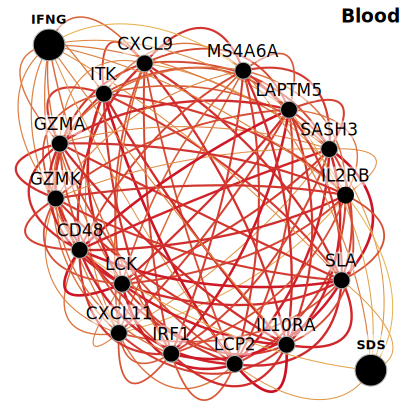
\includegraphics[width=\textwidth]{gene_pair_networks/GIANT-IFNG_vs_SDS-blood.pdf}
     \end{subfigure}
     \hfill
     \begin{subfigure}[b]{0.3\textwidth}
         \centering
         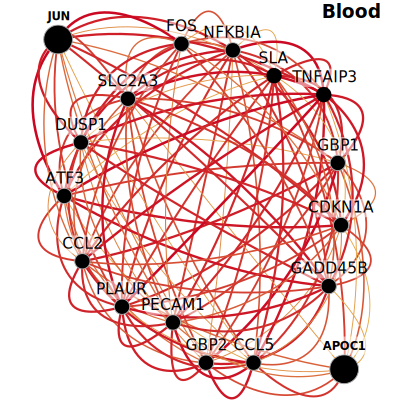
\includegraphics[width=\textwidth]{gene_pair_networks/GIANT-JUN_vs_APOC1-blood.pdf}
         %\label{fig:three sin x}
     \end{subfigure}
     \hfill
     \begin{subfigure}[b]{0.3\textwidth}
         \centering
         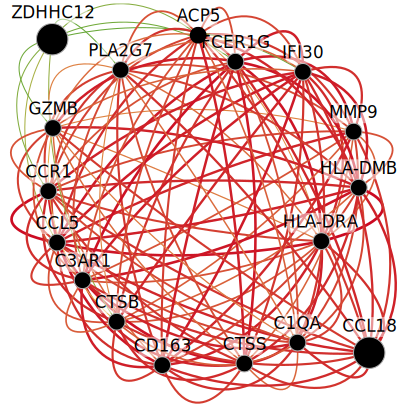
\includegraphics[width=\textwidth]{gene_pair_networks/GIANT-ZDHHC12_vs_CCL18-blood.pdf}
         %\label{fig:three sin x}
     \end{subfigure}
     \hfill
     \begin{subfigure}[b]{0.3\textwidth}
         \centering
         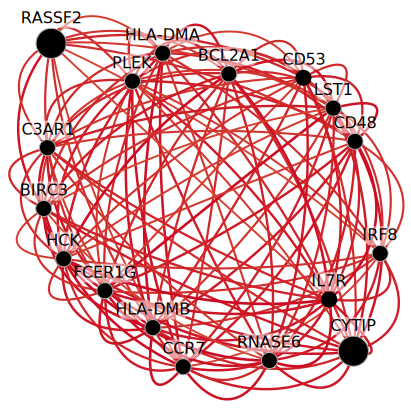
\includegraphics[width=\textwidth]{gene_pair_networks/GIANT-RASSF2_vs_CYTIP-blood.pdf}
         %\label{fig:three sin x}
     \end{subfigure}
     \hfill
     \begin{subfigure}[b]{0.3\textwidth}
         \centering
         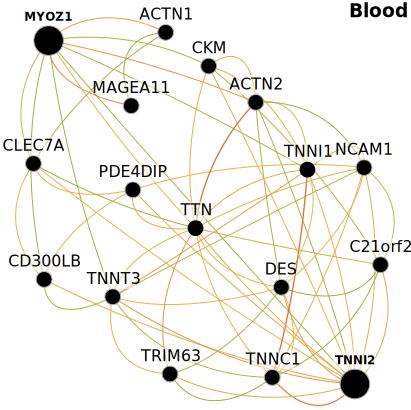
\includegraphics[width=\textwidth]{gene_pair_networks/GIANT-MYOZ1_vs_TNNI2-blood.pdf}
         %\label{fig:three sin x}
     \end{subfigure}
     \hfill
     \begin{subfigure}[b]{0.3\textwidth}
         \centering
         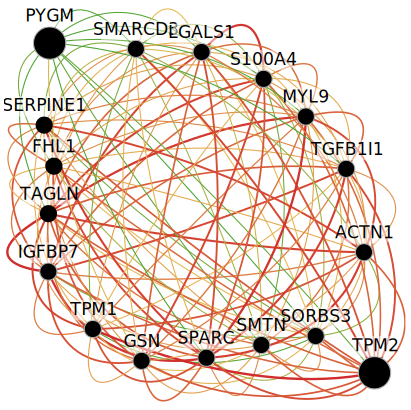
\includegraphics[width=\textwidth]{gene_pair_networks/GIANT-PYGM_vs_TPM2-blood.pdf}
         %\label{fig:three sin x}
     \end{subfigure}
\end{figure}

\begin{tikzpicture}[remember picture,overlay]
    \node[anchor=north east,inner sep=0pt] at ($(current page.north east)+(-5.3cm,-6.1cm)$) {
       
\includegraphics[width=9.5px]{gene_pair_networks/color_bar.pdf}
    };
\end{tikzpicture}

\end{document}

